\section{Cardinalità}
Il concetto di cardinalità è, forse, il modo più semplice di contare gli elementi di un insieme: diciamo che due insiemi hanno un ugual numero di elementi se esiste
una corrispondenza biunivoca fra di essi.

\begin{definition}[Equipotenza/Cardinalità]
	Dati due insiemi $A$ e $B$:
	\[ |A| = |B| \Mydef \exists f \in {}^A B \; \text{``$f$ è bigettiva $A \rightarrow B$''}
		\]
	diciamo anche che ``$A$ ha la stessa \vocab{cardinalità} di $B$'' o che ``$A$ e $B$ sono \vocab{equipotenti}''. Poniamo inoltre:
	\[ |A| \leq |B| \Mydef \exists B' \subseteq B \; |A| = |B'| 
		\]
	ossia $\exists f \in {}^A B$ ``$f$ è iniettiva'' (la definizione ci dice proprio che esiste un sottoinsieme di $B$ che è in bigezione con $A$, e per definizione di iniettività, si ha proprio che $A \hookrightarrow B$)\footnote{Tale relazione sarà anche una relazione di ordine tra cardinalità quando queste ultime saranno singoli oggetti della teoria.}.
\end{definition}

\begin{note}[Sulla notazione per le cardinalità]
	Osserviamo che:
	\begin{itemize}
		\item La scrittura $|A| = |B|$ suggerisce che esistono insiemi - o oggetti di qualche genere - denotati $|A|$ e $|B|$ di cui si predica l'uguaglianza.
		Effettivamente costruiamo questi oggetti, ma, per ora, la scrittura $|A| = |B|$ è inscindibile, come \ding{168}$[A,B)$ (nel senso che per ora è solo un'abbreviazione per dire bigezione, pertanto non possiamo separare quei simboli o farci qualcosa).
		\item Potrebbe sorgere il sospetto che se $|A|\textcolor{red}{<}|B|$ quando $A \subsetneq B$, ma non è così, come mostra l'esempio di $A = \{x \in \omega | x > 0\}$ e $B = \omega$, infatti $A \subsetneq B$, ma $|A| = |B|$.
	\end{itemize}
\end{note}

\begin{remark}[Proprietà formali di una relazione di equivalenza]
	La relazione $|\cdot| = |\cdot|$ soddisfa le proprietà formali di una relazione di equivalenza (ma per ora NON lo è\footnote{Potrebbe tuttavia essere pensata come una relazione di equivalenza su $V$ (la classe di tutti gli insiemi).}):
	\begin{itemize}
		\item \textbf{riflessività}: $|A| = |A|$.
		\item \textbf{simmetria}: $|A| = |B| \rightarrow |B| = |A|$.
		\item \textbf{transitività}: $|A| = |B| \land |B| = |C| \rightarrow |A| = |C|$.
	\end{itemize}
\end{remark}

\begin{exercise}
	Dimostrare l'osservazione.
\end{exercise}

\begin{soln}
Per la riflessività basta osservare che $\id_A$ è una bigezione da $A$ in $A$. Per la simmetria, abbiamo visto che se $f : A \rightarrow B$ è iniettiva, allora ammette
inversa $g : \Imm(f) \rightarrow A$ a sua volta iniettiva (e surgettiva poiché ha necessariamente come immagine tutto $A$), inoltre, essendo $f$ bigettiva si ha che $\Imm(f) = B$, quindi $g : B \rightarrow A$, e 
per quanto detto è bigettiva, dunque nel linguaggio della cardinalità $|B| = |A|$.\\
Infine, $|A| = |B| \iff \exists f : A \rightarrow B$ bigettiva, $|B| = |C| \iff \exists g : B \rightarrow C$ bigettiva, ora è sufficiente osservare che $g \circ f : A \rightarrow C$ è bigettiva in quanto composizione di funzioni bigettive\footnote{È una semplice verifica.}, per avere $|A| = |C|$.
\end{soln}

\begin{remark}[Proprietà formali $\lbrack$parziali$\rbrack$ di una relazione di ordine $\lbrack$largo$\rbrack$]
	La relazione $|\cdot| \leq |\cdot|$ soddisfa\footnote{Tali proprietà, unite al teorema di Cantor-Bernstein, che stiamo per vedere, ci danno una relazione di ordine totale su $V$.}:
	\begin{itemize}
		\item \textbf{riflessività}: $|A| \leq |A|$.
		\item \textbf{transitività}: $|A| \leq |B| \land |B| \leq |C| \rightarrow |A| \leq |C|$.
	\end{itemize}
\end{remark}

\begin{exercise}
	Dimostrare l'osservazione.
\end{exercise}

\begin{soln}
Per la riflessività basta osservare che $\id_A$ è in particolare una mappa iniettiva (oppure che $A$ è un sottoinsieme [improprio] di se stesso e quindi l'identità è la bigezione richiesta dalla definizione).
Per la transitività $|A| \leq |B| \iff \exists A \hookrightarrow B$, $|B| \leq |C| \iff \exists g : B \hookrightarrow C$, e osservando che la composizione di funzioni iniettive è iniettiva, si ha che $g \circ f : A \rightarrow C$ è iniettiva $\iff |A| \leq |C|$.
\end{soln}

Per stabilire che le cardinalità sono, formalmente, ordinate dalla relazione $|\cdot| \leq |\cdot|$, ci manca l'antisimmetria, che è appunto enunciata dal teorema seguente.

\subsection{Teorema di Cantor-Bernstein}

\begin{theorem}
	[Cantor-Bernstein]
	\label{CB}
	Se c'è una funzione iniettiva $A \rightarrow B$ e una funzione iniettiva $B \rightarrow A$, allora esiste una bigezione fra $A$ e $B$.
	\[ \forall A,B (|A| \leq |B| \land |B| \leq |A|) \rightarrow |A| = |B|
		\]
\end{theorem}

\begin{proof}
	Per ipotesi abbiamo quindi $f: A \rightarrow B$ e $g: B \rightarrow A$ iniettive. Il nostro obiettivo è costruire una nuova funzione $h : A \rightarrow B$ bigettiva.\\
	\textcolor{MidnightBlue}{L'idea è che ogni elemento, poniamo, di $A$, è una tappa di un percorso:
	\[ a \overset{f}{\to} f(a) \overset{g}{\to} g(f(a)) \overset{f}{\to} f(g(f(a))) \overset{g}{\to} \dots
		\]
	Siccome $f$ e $g$ sono iniettive, questo percorso ha altresì un'unica estensione all'indietro - sappiamo che se le funzioni sono iniettive, allora ammettono un'inversa iniettiva (e surgettiva verso l'insieme di partenza),
	dunque possiamo sempre tornare indietro in modo unico, estendendo quindi il nostro percorso anche nell'altra direzione:
	\[ \ldots\overset{g}{\to}\textcolor{red}{f^{-1}(g^{-1}(a))} \overset{f}{\to} \textcolor{red}{g^{-1}(a)} \overset{g}{\to} a \overset{f}{\to} f(a) \overset{g}{\to} g(f(a)) \overset{f}{\to} f(g(f(a))) \overset{g}{\to} \ldots
		\]
	a patto che $a \in \Imm(g)$ (poiché $g^{-1} : A \supseteq \Imm(g) \to B$ - ed è bigettiva), $g^{-1}(a) \in \Imm(f)$, etc. Quando, e se, non possiamo più applicare la funzione inversa, il percorso (all'indietro) si interrompe.
	Con questa catena di composizioni osserviamo che ci sono quindi solo tre tipi di percorsi possibili:
	\begin{figure}[H]
		\centering
		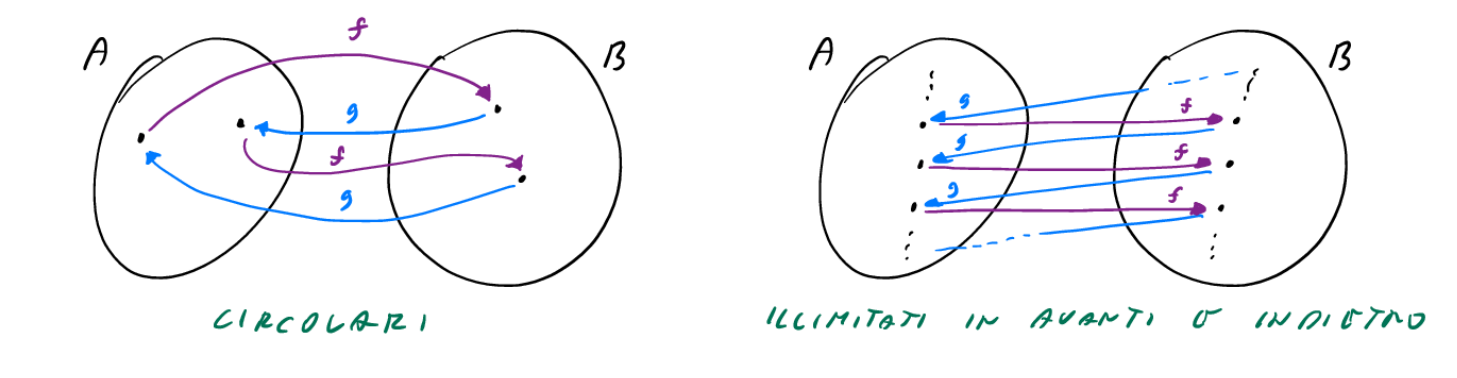
\includegraphics[width=12.5cm]{immagini/cantor-ber1a.png}
	\end{figure}
	\begin{figure}[H]
		\centering
		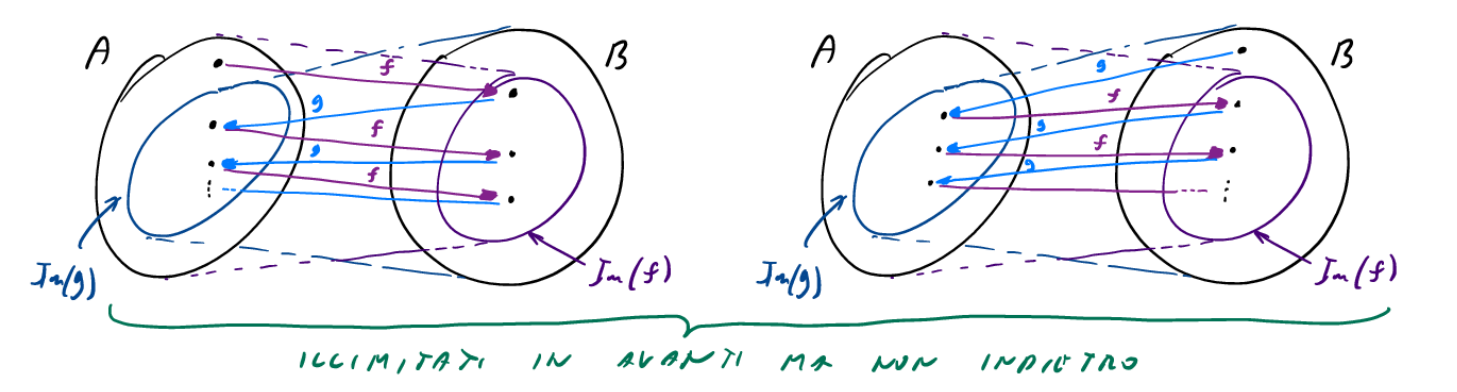
\includegraphics[width=12.5cm]{immagini/cantor-ber1b.png}
	\end{figure}
	Per gli elementi che si trovano su un percorso circolare, o su un percorso illimitato avanti e indietro, $f$ fornisce una bigezione, come la fornirebbe anche $g^{-1}$ - la scelta è arbitraria a patto di 
	usare la medesima funzione per l'intero percorso - nel modo seguente\footnote{Informalmente, se siamo in uno dei due casi, allora $f$ è per forza una mappa bigettiva, perché è iniettiva e ``prende'' tutti gli elementi in arrivo, idem $g^{-1}$.}:
	\begin{figure}[H]
		\centering
		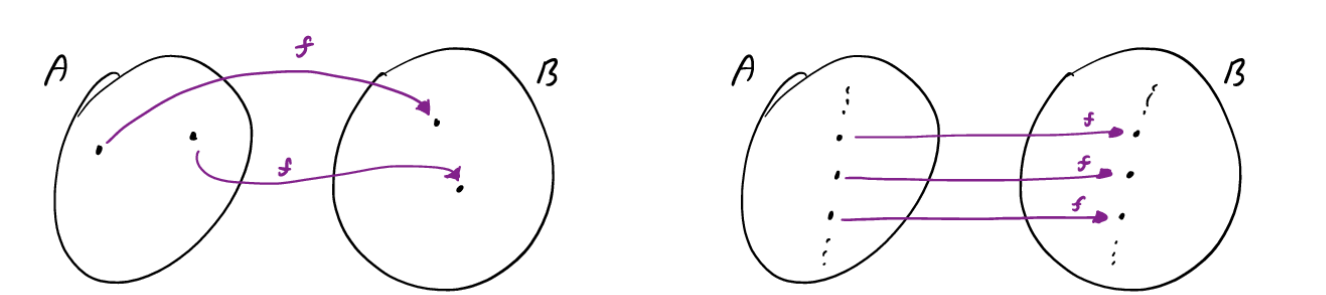
\includegraphics[width=12.5cm]{immagini/cantor-ber2a.png}
	\end{figure}
	\begin{figure}[H]
		\centering
		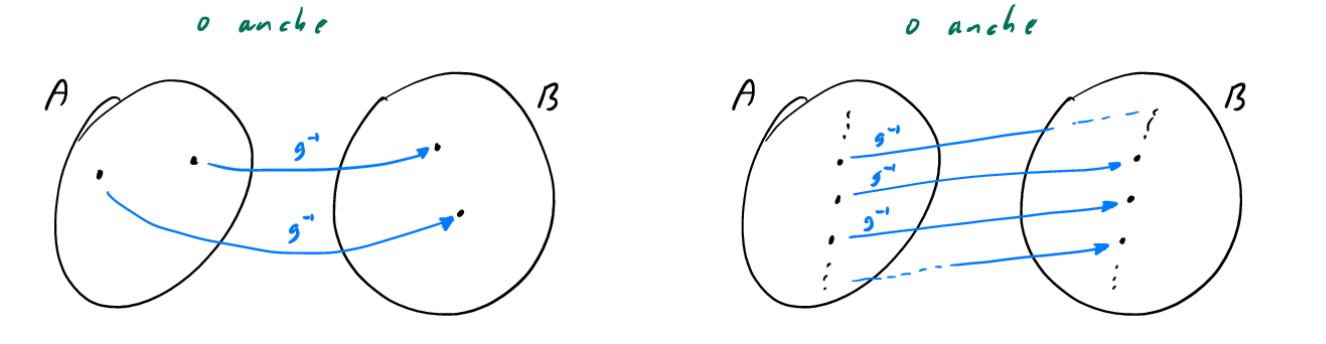
\includegraphics[width=11.5cm]{immagini/cantor-ber2b.png}
	\end{figure}
	Per i percorsi illimitati solo in avanti, occorre invece vedere in quale insieme sta l'elemento iniziale del percorso: se questo è in $A$, la bigezione è data da $f$,
	altrimenti se sta in $B$ la bigezione è data da $g^{-1}$.
	\begin{figure}[H]
		\centering
		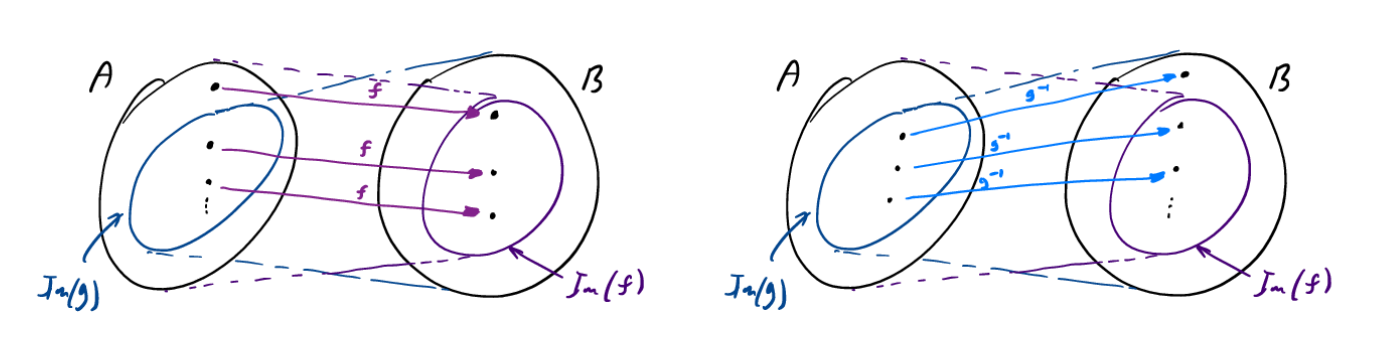
\includegraphics[width=12.5cm]{immagini/cantor-ber3.png}
	\end{figure}
	Per comodità poniamo quindi $h(x) = f(x)$ in ogni caso, eccetto quando $x$ è lungo un percorso che parte da $B$, nel cui caso poniamo $h(x) = g^{-1}(x)$.}\\
	Formalmente, definiamo per \hyperref[ric1]{ricorsione} (prima forma) le seguenti successioni di sottoinsiemi di $B$ e $A$ rispettivamente - ossia, tecnicamente, la funzione $\omega \rightarrow \ps(B) \times \ps(A) : i \mapsto (B_i,A_i)$, con:
	\[ B_0 = B \setminus\Imm(f) \qquad A_i = g[B_i] \qquad B_{s(i)} = f[A_i]
		\]
	Definiamo quindi:
	\[ B_* = \bigcup_{i \in \omega}B_i \Mydef \bigcup\{B_i | i \in \omega\} \qquad A_* = \bigcup_{i \in \omega} A_i
		\]
	Questi sono i punti che appartengono a cammini che partono da $B$, definiamo quindi $h : A \rightarrow B$ e $k : B \rightarrow A$ come segue:
	\[ h(x) = \begin{cases}
		g^{-1}(x) &\text{se $x \in A_*$}\\
		f(x) &\text{altrimenti}
	\end{cases}
	\qquad
	k(y) = \begin{cases}
		g(y) &\text{se $y \in B_*$}\\
		f^{-1}(y) &\text{altrimenti}
	\end{cases}
		\]
	\textcolor{purple}{queste mappe coprono tutti i casi  possibili, infatti, i percorsi ciclici e illimitati da entrambe le parti sono coperti da $k = f^{-1}$ ed $h = g^{-1}$, mentre nel caso di percorsi che partono da $B$ e sono limitati a sinistra [all'indietro], ovvero con primo elemento in $B^*$ abbiamo che $k(y) = g(y)$,
	invece nel caso simmetrico, in cui si parte da $A$ con percorso limitato a sinistra (quindi $x \not \in A_*$) si ha $h(x) = f(x)$, in tal modo prendiamo tutti gli elementi di entrambi gli insiemi, ed essendo che $f$ e $g$ sono iniettive, per ipotesi, non rischiamo sovrapposizioni ed otteniamo proprio delle bigezioni.}\\
	Ci basta quindi dimostrare che $h$ e $k$ sono ben definite, $k \circ h = \id_A$ e $h \circ k = \id_B$, in tal modo avremo la nostra bigezione (e la sua inversa).
	\begin{itemize}
		\item[$\boxed{\text{$h$ e $k$ ben definite}}$] Occorre verificare che stiamo applicando $g^{-1}$ e $f^{-1}$ a elementi della immagine di $g$ e $f$ rispettivamente.
		Nella definizione di $h$, se $x \in A_*$, allora $x \in A_i$, per qualche $i \in \omega$, quindi $x \in g[B_i] \subseteq \Imm(g)$. Nella definizione di $k$, se $y \not \in B_*$, in particolare,
		$y \not \in B_0$, per cui $y \in \Imm(f)$.
		\item[$\boxed{k \circ h = \id_A}$] Se $x \in A_*$, allora $x \in A_i$, per qualche $i \in \omega$, quindi $x = g(y)$, con $y \in B_i$, per cui $k(h(y)) = k(g^{-1}(x)) = k(y) = g(y) = x$ (abbiamo usato che $y = g^{-1}(x) \in B_*$ per quanto supposto sopra).\\
		Per il caso $x \not \in A_*$, osserviamo, intanto, che $x \not \in A_* \implies f(x) \not \in B_*$. Infatti, se $f(x) \in B_i$, con $i \in \omega$, allora $i \ne 0$, perché $B_0 = B \setminus \Imm(f)$, quindi possiamo scrivere $i = s(j)$, 
		e $f(x) \in B_{s(j)} = f[A_j]$. Per l'iniettività di $f$, abbiamo allora $x \in A_j \;\lightning$\\
		Di conseguenza, se $x \not \in A_*$, $k(h(x)) = k(f(x)) \overset{f(x) \not \in B_*}{=} f^{-1}(f(x)) = x$.
		\item[$\boxed{h \circ k = \id_B}$] Se $y \in B_*$, allora $y \in B_i$, per qualche $i \in \omega$, quindi $g(y) \in A_i$. Di conseguenza $h(k(y)) = h(g(y)) = g^{-1}(g(y)) = y$. Altrimenti $y \not \in B_*$ e, se $f^{-1}(y)\in A_*$, avremmo una contraddizione,
		perché $f^{-1}(y) \in A_i \rightarrow y = f(f^{-1}(y)) \in A_{s(i)}$. Quindi $h(k(y)) = h(f^{-1}(y)) = f(f^{-1}(y)) = y$.
	\end{itemize}
\end{proof}

Visto che $|\cdot|\leq|\cdot|$ ha le proprietà formali di una relazione d'ordine fra le classi di equivalenza della relazione $|\cdot| = |\cdot|$, possiamo definire il corrispondente ordine stretto.

\begin{definition}[Ordinamento stretto fra cardinalità]
	Dati due insiemi $A$ e $B$ definiamo:
	\[ |A| < |B| \Mydef |A| \leq |B| \land |A| \ne |B| \, \footnote{Dove ricordiamo che $|A| \ne |B| \Mydef \neg(|A| = |B|)$.}
		\]
\end{definition}

\subsection{Teorema di Cantor}

\begin{theorem}[Cantor]
	\label{cantor}
	Dato un qualunque insieme $A$ vale:
	\[ |A| < |\ps(A)|
		\]
\end{theorem}

La dimostrazione di questo enunciato è, ancora una volta, il medesimo argomento del paradosso di Russell.

\begin{proof}
	La disuguaglianza $|A| \leq |\ps(A)|$ è facile: basta considerare la funzione iniettiva:
	\[ A \to \ps(A) : x \mapsto \{x\}
		\]
	(che è iniettiva per \hyperref[ax2]{estensionalità}). Consideriamo, ora, una qualunque funzione $f : A \rightarrow \ps(A)$ iniettiva.
	Dobbiamo dimostrare che $\Imm(f) \subsetneq \ps(A)$ (cioè che non è surgettiva). Consideriamo:
	\[ B = \{x \in A | x \not \in f(x)\} \, \footnote{$f(x) \in \ps(A)$, ovvero è un sottoinsieme di $A$, quindi stiamo considerando il sottoinsieme degli elementi di $A$ che non stanno nelle loro immagini (dei sottoinsiemi di $A$).}
		\]
	Ora $B \subseteq A$, supponendo per assurdo che $f$ sia bigettiva, ovvero che $B = f(a)$ per qualche $a \in A$, avremmo:
	\[ a \in f(a) \subseteq A \iff a \in B \iff a \not \in f(a) \; \lightning
		\]
\end{proof}

\subsection{Operazioni fra cardinalità}

\begin{definition}[Somma, prodotto e potenze di cardinalità]
	Dati $A$ e $B$ possiamo definire somma, prodotto e potenze di cardinalità come segue:
	\[ \begin{split}
		|A| + |B| &\Mydef |A \sqcup B| \Mydef |(A \times \{0\}) \cup (B \times \{1\})| \\
		|A|\cdot |B| &\Mydef |A \times B| \\
		|A|^{|B|} &\Mydef |{}^{B}A|
	\end{split}
		\]
	(nella definizione di unione disgiunta abbiamo fatto il prodotto per cose diverse, in modo che gli elementi comuni ai due insiemi sono comunque diversi per la seconda componente, e quindi siano contati due volte.)
\end{definition}

Osserviamo che le operazioni fra cardinalità così date sono ben definite.

\begin{proposition}[Buona definizione delle operazioni]
	Le operazioni di somma, prodotto e potenza fra cardinalità sono ben definite modulo bigezioni, ossia dati $A,B,A',B'$, con $|A| = |A'|$ e $|B| = |B'|$, vale:
	\[ |A| + |B| = |A'| + |B'| \qquad |A|\cdot|B| = |A'|\cdot|B'| \qquad |A|^{|B|} = |A'|^{|B'|}
		\]
\end{proposition}

\begin{proof}
	Date $f : A \rightarrow A'$ e $g : B \rightarrow B'$ bigettive, è immediato verificare che le seguenti sono bigezioni:
	\[  \begin{split}
		A \sqcup B \to A' \sqcup B' :\,& (a,0) \mapsto (f(a),0) \\
											 \,& (b,1) \mapsto (g(b),1) \\
	 	A \times B \to A' \times B' :\,& (a,b) \mapsto (f(a),g(b)) \\
		{}^{B}A \to {}^{B'}A' :\,& h \mapsto f \circ h \circ g^{-1} \, \footnote{Deriva dal diagramma commutativo che si può disegnare.}
		\end{split}
		\]
	ed equivalgono alle uguaglianze di cardinalità nella tesi.
\end{proof}

\begin{notation}[Cardinalità finite]
Riferendoci alle cardinalità finite $|\emptyset|,|1|,|2|,\ldots$ se non c'è rischio di confusione, scriveremo semplicemente $0,1,2,\ldots$
\end{notation}

\begin{remark}[Teorema di Cantor rivisitato]
	$|\ps(A)| = 2^{|A|}$, per cui il \hyperref[cantor]{teorema di Cantor}, può essere enunciato dicendo che, dato un qualunque $A$, vale $|A| < 2^{|A|}$.
\end{remark}

Verifichiamo che effettivamente ci sia una bigezione tra l'insieme delle parti di $A$ e quello delle funzioni da $A$ in 2.

\begin{proof}
	La funzione che ad ogni $B \in \ps(A)$ associa la sua \vocab{funzione indicatrice} $\chi_B : A \rightarrow 2$ è definita da:
	\[ \chi_B(x) = \begin{cases}
		1 &\text{se $x \in B$}\\
		0 &\text{altrimenti}
	\end{cases}
		\]
	ed è una bigezione $\ps(A) \rightarrow {}^{A}2$ (ovvero $|\ps(A)| = |{}^{A}\{0,1\}| = |{}^{A}2|$ per la nostra codifica dei naturali, e per la definizione data prima la seconda cardinalità corrisponde proprio all'operazione $|2|^{|A|}$).
\end{proof}

\begin{proposition}[Proprietà delle operazioni fra cardinalità]
	Le operazioni fra cardinalità godono delle proprietà seguenti: denotando, per brevità, con $\alpha,\beta,\gamma$ i simboli: $|A|,|B|,|C|$:
	\begin{align*}
		&\alpha + 0 = \alpha 	 & \quad & \alpha + \beta = \beta + \alpha 		 	& \quad & \alpha + (\beta + \gamma) = (\alpha + \beta) + \gamma \\
		&\alpha \cdot 0 = 0 	 & \quad & \alpha \cdot \beta = \beta \cdot \alpha 	& \quad & \alpha \cdot (\beta \cdot \gamma) = (\alpha \cdot \beta) \cdot \gamma \\
		&\alpha \cdot 1 = \alpha & \quad & \alpha \cdot (\beta + \gamma) = \alpha \cdot \beta + \alpha \cdot \gamma \\
		&\alpha^0 = 1 			 & \quad & (\alpha^\beta)^\gamma = \alpha^{\gamma \cdot \beta} & \quad & (\alpha \cdot \beta)^\gamma = \alpha^\gamma \cdot \beta^\gamma \\
		&1^\alpha = 1			 & \quad & \alpha^{\beta + \gamma} = \alpha^\beta \cdot \alpha^\gamma
	\end{align*}
\end{proposition}

\begin{proof}
	In ciascun caso, si tratta semplicemente di esibire una bigezione esplicita fra il membro di sinistra e il membro di destra. Come esempio, vediamo uno dei casi più complicati, il resto 
	è lasciato come \textcolor{red}{esercizio}. \\
	Dimostriamo che $(|A|^{|B|})^{|C|} = |A|^{|C|\cdot|B|}$. Dobbiamo esibire una bigezione fra l'insieme ${}^C({}^BA)$ delle funzioni che ad ogni elemento di $C$ associano una funzione $B \rightarrow A$, e l'insieme ${}^{C \times B}A$, delle funzioni 
	che ad ogni coppia di elementi in $C \times B$ associano un elemento di $A$. Associamo a $f \in {}^C({}^BA)$ la funzione $\widetilde{f} \in {}^{C \times B}A$ definita da:
	\[ \widetilde{f}(c,b) = (\underbrace{f(c)}_{\in {}^{B}A})(\underbrace{b}_{\in B}) \, \footnote{Cioè la mappa $\sim$ prende una funzione da $C$ a ${}^{B}A$ e la manda in un'altra che prende coppie di elementi in $C \times B$, e valuta il primo elemento in $f$ 
	per ottenere una mappa da $B$ a $A$, che poi valuta in $b \in B$.}
		\]
	Dimostriamo che l'inversa di questa applicazione associa a $g \in {}^{C \times B}A$ la funzione $\overline{g} \in {}^{C}({}^B A)$ definita da:
	\[	\overline{g}(c) : B \to A : b \mapsto g(c,b) \, \footnote{Ovvero la mappa $-$ associa una mappa di ${}^{C\times B}A$ con la mappa $\overline{g} \in {}^{C}({}^B A)$, che valutata in $c \in C$, dà una funzione da $B$ in $A$, che ad ogni $b \in B$ associa $g(c,b)$.}
		\]
	La verifica è facilissima, presa $g \in {}^{C \times B}A$ si ha:
	\[ \forall (c,b) \in C \times B \quad \widetilde{\overline{g}}(c,d) = (\overline{g}(c))(b) = g(c,b) \implies \widetilde{\overline{g}} = g
		\]
	(quindi $\sim \circ -$ è l'identità). Presa $f \in {}^{C}({}^B A)$, e fissato un qualunque $c \in C$, si ha:
	\[ \forall b \in B \,(\overline{\widetilde{f}}(c)(b)) = \widetilde{f}(c,b) = (f(c))(b) \implies \overline{\widetilde{f}}(c) = f(c)
		\]
	da cui, per l'arbitrarietà di $c$, $\overline{\widetilde{f}} = f$ (e quindi $- \circ \sim$ è l'identità).
\end{proof}